% presentation_v2_eng.tex
% Beamer slides for the oral presentation — Perceiver Project (V2 English)
% Compile with: pdflatex presentation_v2_eng.tex (x2 for TOC)

\documentclass[aspectratio=169,11pt]{beamer}

% ── Theme and Colors ─────────────────────────────────────────────────────────
\usetheme{Madrid}
\usecolortheme{default}

\definecolor{UnifiBlue}{RGB}{0,82,147}
\definecolor{UnifiDark}{RGB}{33,37,41}
\definecolor{AccentOrange}{RGB}{230,126,34}
\definecolor{AccentGreen}{RGB}{39,174,96}
\definecolor{AccentRed}{RGB}{231,76,60}

% Apply colors to theme
\setbeamercolor{structure}{fg=UnifiBlue}
\setbeamercolor{title}{fg=white, bg=UnifiBlue}
\setbeamercolor{frametitle}{fg=white, bg=UnifiBlue}
\setbeamercolor{itemize item}{fg=UnifiBlue}
\setbeamercolor{itemize subitem}{fg=UnifiBlue!80}
\setbeamercolor{block title}{bg=UnifiBlue, fg=white}
\setbeamercolor{block body}{bg=UnifiBlue!10, fg=UnifiDark}
\setbeamercolor{block title alerted}{bg=AccentRed, fg=white}
\setbeamercolor{block body alerted}{bg=AccentRed!10, fg=UnifiDark}
\setbeamercolor{block title example}{bg=AccentGreen, fg=white}
\setbeamercolor{block body example}{bg=AccentGreen!10, fg=UnifiDark}
\setbeamercolor{alerted text}{fg=AccentOrange}

% Remove navigation symbols
\setbeamertemplate{navigation symbols}{}

% Footer format
\setbeamertemplate{footline}{%
  \leavevmode\hbox{%
    \begin{beamercolorbox}[wd=.42\paperwidth,ht=2.5ex,dp=1ex,center]{author in head/foot}%
      \usebeamerfont{author in head/foot}\scriptsize\insertshortauthor
    \end{beamercolorbox}%
    \begin{beamercolorbox}[wd=.40\paperwidth,ht=2.5ex,dp=1ex,center]{title in head/foot}%
      \usebeamerfont{title in head/foot}\scriptsize\insertshorttitle
    \end{beamercolorbox}%
    \begin{beamercolorbox}[wd=.18\paperwidth,ht=2.5ex,dp=1ex,right]{date in head/foot}%
      \usebeamerfont{date in head/foot}\scriptsize\insertframenumber{}/\inserttotalframenumber\hspace*{2ex}
    \end{beamercolorbox}%
  }%
}

% ── Packages ─────────────────────────────────────────────────────────────────
\usepackage[utf8]{inputenc}
\usepackage[T1]{fontenc}
\usepackage[english]{babel}
\usepackage{graphicx}
\usepackage{booktabs}
\usepackage{amsmath,amssymb}
\usepackage{multirow}
\usepackage{tikz}
\usepackage{pgfplots}
\usepackage{hyperref}
\usepackage{fontawesome5}

\usetikzlibrary{arrows.meta,positioning,calc,fit,backgrounds,shapes.geometric,decorations.pathreplacing}
\pgfplotsset{compat=1.18}

% ── Figure Paths ─────────────────────────────────────────────────────────────
\graphicspath{
  {charts/}
  {../Perceiver_Paper/figures/}
  {../Perceiver_Paper/analysis_results/}
  {../Perceiver_Paper/attention_analysis/}
  {../Perceiver_Paper/perceiver_visualizations/}
}

% ── Metadata ─────────────────────────────────────────────────────────────────
\title[Perceiver \& Perceiver IO]{Perceiver \& Perceiver IO}
\subtitle{Implementation and Experimental Analysis}
\author[F.Gigli C.Vignoli]{Francesco Gigli e Corso Vignoli}
\institute[UNIFI]{Universit\`a degli Studi di Firenze\\Course B031278 --- Deep Learning}
\date{}

\newcommand{\AgendaItem}[2]{%
  \noindent
  \begin{tikzpicture}[baseline=(n.base)]
    \node[
      circle,
      shade,
      ball color=UnifiBlue!85,
      text=white,
      minimum size=1.8em,
      inner sep=0pt,
      font=\bfseries\small
    ] (n) {#1};
  \end{tikzpicture}%
  \hspace{0.8em}{\color{UnifiBlue}\LARGE #2}\par\vspace{1.15em}
}

% ══════════════════════════════════════════════════════════════════════════════
\begin{document}

% ══════════════════════════════════════════════════════════════════════════════
% SECTION 1: Introduction & Motivation (slides 1-5)
% ══════════════════════════════════════════════════════════════════════════════

% ── Slide 1: Title ───────────────────────────────────────────────────────────
\begin{frame}
  \titlepage
\end{frame}

% ── Slide 2: Agenda ──────────────────────────────────────────────────────────
\begin{frame}{Agenda}
  \vspace{1.3em}
  \AgendaItem{1}{Introduction \& Motivation}
  \AgendaItem{2}{Perceiver: Architecture, FFN, Weight Sharing}
  \AgendaItem{3}{Perceiver: Experiments \& Results}
  \AgendaItem{4}{Perceiver IO: Decoder, Queries, Results}
\end{frame}

% ══════════════════════════════════════════════════════════════════════════════
\section{Introduction \& Motivation}
% ══════════════════════════════════════════════════════════════════════════════

% ── Slide 3: The Problem ─────────────────────────────────────────────────────
\begin{frame}[shrink=10]{The Problem: Modality-Specific Architectures}
  \begin{columns}[T,onlytextwidth]
    \begin{column}{0.56\textwidth}
      {\color{UnifiBlue}\large\bfseries One modality, one architecture}

      \vspace{0.65em}
      \begin{center}
      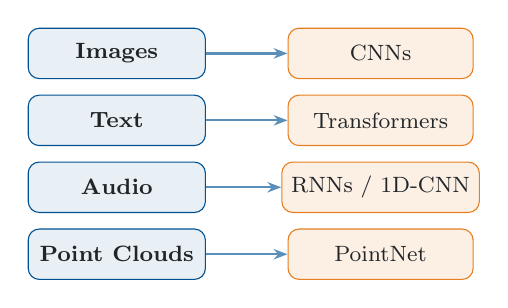
\begin{tikzpicture}[
        modbox/.style={rectangle, draw=UnifiBlue, fill=UnifiBlue!9,
                       rounded corners=4pt, minimum width=2.25cm, minimum height=0.64cm,
                       font=\footnotesize\bfseries, text=UnifiDark},
        archbox/.style={rectangle, draw=AccentOrange, fill=AccentOrange!12,
                        rounded corners=4pt, minimum width=2.35cm, minimum height=0.64cm,
                        font=\footnotesize, text=UnifiDark},
        myarrow/.style={-{Stealth[length=5pt]}, thick, UnifiBlue!65}
      ]
        \node[modbox] (img) at (0,0) {Images};
        \node[modbox] (txt) at (0,-0.85) {Text};
        \node[modbox] (aud) at (0,-1.70) {Audio};
        \node[modbox] (pc)  at (0,-2.55) {Point Clouds};

        \node[archbox] (cnn)   at (3.35,0) {CNNs};
        \node[archbox] (trans) at (3.35,-0.85) {Transformers};
        \node[archbox] (rnn)   at (3.35,-1.70) {RNNs / 1D-CNN};
        \node[archbox] (pnet)  at (3.35,-2.55) {PointNet};

        \draw[myarrow] (img) -- (cnn);
        \draw[myarrow] (txt) -- (trans);
        \draw[myarrow] (aud) -- (rnn);
        \draw[myarrow] (pc)  -- (pnet);
      \end{tikzpicture}
      \end{center}

      \vspace{0.35em}
      \small
      Each data type is usually paired with a dedicated model and
      domain-specific assumptions about structure.
    \end{column}

    \begin{column}{0.40\textwidth}
      {\color{UnifiBlue}\large\bfseries The scaling bottleneck}

      \vspace{0.45em}
      \begin{block}{Self-attention cost}
        \centering
        {\Large $\mathcal{O}(M^2 \cdot d)$}\\[0.2em]
        {\scriptsize grows quadratically with input length $M$}
      \end{block}

      \vspace{0.35em}
      \begin{table}
        \centering\small
        \begin{tabular}{lr}
          \toprule
          \textbf{Input representation} & \textbf{$M$} \\
          \midrule
          $16\!\times\!16$ image patches & $256$ \\
          raw $224\!\times\!224$ pixels & $50{,}176$ \\
          \bottomrule
        \end{tabular}
      \end{table}

      \vspace{0.15em}
      \centering\small
      Raw pixels make standard attention \alert{impractical}.
    \end{column}
  \end{columns}

  \vspace{1.1em}
  {\color{UnifiBlue!25}\hrule height 0.6pt}
  \vspace{0.6em}
  \centering\small
  {\color{UnifiBlue}\textbf{Core question:}}\, can one architecture handle arbitrary inputs without quadratic cost?
\end{frame}

\newcommand{\SolutionCard}[3]{%
  \begin{beamercolorbox}[wd=\linewidth,rounded=true,shadow=true,sep=0pt]{solution card body}
    \begin{beamercolorbox}[wd=\linewidth,rounded=true,sep=0.06cm,leftskip=0.16cm]{solution card title}
      {\normalsize #1}
    \end{beamercolorbox}
    \vspace{0.10em}
    \hspace{0.16cm}\begin{minipage}[t][0.74cm][t]{0.88\linewidth}
      \raggedright
      \hyphenpenalty=10000\exhyphenpenalty=10000
      {\scriptsize\bfseries #2}\\[-0.10em]
      {\scriptsize #3}
    \end{minipage}
    \vspace{0.10em}
  \end{beamercolorbox}%
}

% ── Slide 4: The Perceiver Solution ──────────────────────────────────────────
\begin{frame}[shrink=5]{The Perceiver Solution}
  \setbeamercolor{solution card title}{bg=UnifiBlue, fg=white}
  \setbeamercolor{solution card body}{bg=UnifiBlue!8, fg=UnifiDark}
  \small
  \begin{center}
    \begin{minipage}{0.88\textwidth}
      \centering
      {\color{UnifiBlue}\textbf{Core idea:}} learned latents read the input once; expensive processing stays in latent space.
    \end{minipage}
  \end{center}

  \vspace{0.80em}
  \noindent
  \begin{minipage}[t]{0.29\textwidth}
    \SolutionCard{1. Read}{Cross-attention}{$M$ inputs $\to$ $N \ll M$ latents}
  \end{minipage}\hfill
  \begin{minipage}[t]{0.29\textwidth}
    \SolutionCard{2. Process}{Latent block}{transform $N$ latent slots}
  \end{minipage}\hfill
  \begin{minipage}[t]{0.29\textwidth}
    \SolutionCard{3. Reuse}{Shared weights}{repeat the same processor}
  \end{minipage}

  \vspace{0.22em}
  \begin{center}
    {\color{UnifiDark}\bfseries Complexity shift}

    \vspace{0.18em}
    {\footnotesize Read the full input once; repeat the expensive work in the compact latent space $N \ll M$.}

    \vspace{0.24em}
    \scriptsize
    \renewcommand{\arraystretch}{1.04}
    \begin{tabular*}{0.66\textwidth}{@{\extracolsep{\fill}}lc}
      \toprule
      \textbf{Operation} & \textbf{Cost} \\
      \midrule
      Read input once & $\mathcal{O}(M \cdot N)$ \\
      Process latents for $L$ layers & $\mathcal{O}(L \cdot N^2)$ \\
      \midrule
      \textbf{Perceiver} & $\mathcal{O}(M N + L N^2)$ \\
      \bottomrule
    \end{tabular*}
  \end{center}
\end{frame}

% ── Slide 5: Perceiver IO ───────────────────────────────────────────────────
\section{Perceiver Architecture}

\begin{frame}[shrink=5]{Perceiver Architecture}
  \begin{center}
    
\includegraphics[width=0.98\textwidth,height=0.39\textheight,keepaspectratio]{perceiver_arch.png}
  \end{center}

  \vspace{0em}
  \small
  \begin{columns}[T,onlytextwidth]
    \begin{column}{0.50\textwidth}
      \textbf{Encode and process}
      \begin{itemize}
        \item $X \in \mathbb{R}^{M \times C}$ supplies keys and values.
        \item $Z \in \mathbb{R}^{N \times D}$ supplies queries, with $N \ll M$.
        \item Cross-attention maps $X \rightarrow Z$: $\mathcal{O}(M N)$.
      \end{itemize}
    \end{column}

    \begin{column}{0.46\textwidth}
      \textbf{Latent core and output}
      \begin{itemize}
        \item Latent Transformer updates $Z$ only.
        \item Repeated blocks may share weights.
        \item Original Perceiver pools $Z$; Perceiver IO uses output queries.
      \end{itemize}
    \end{column}
  \end{columns}
\end{frame}

% ══════════════════════════════════════════════════════════════════════════════
% SECTION 2: Architecture (slides 5-13)
% ══════════════════════════════════════════════════════════════════════════════
% Section marker moved before the merged architecture slide.

% ── Slide 6: Architecture Overview ───────────────────────────────────────────
% ── Slide 7: Cross-Attention ─────────────────────────────────────────────────
\begin{frame}{Cross-Attention: The Key Mechanism}
  \begin{columns}[T]
    \begin{column}{0.48\textwidth}
      \textbf{Formally:}
      \begin{align*}
        Q &= X_{\text{latent}} \, W_Q \in \mathbb{R}^{N \times d_k} \\
        K &= X_{\text{input}} \, W_K \in \mathbb{R}^{M \times d_k} \\
        V &= X_{\text{input}} \, W_V \in \mathbb{R}^{M \times d_v}
      \end{align*}
      \[
      \text{CrossAttn}(Q,K,V) = \text{softmax}\!\left(\frac{QK^\top}{\sqrt{d_k}}\right) V
      \]

      \vspace{0.3em}
      The \alert{latents are the queries}, the input provides keys and values $\Rightarrow$ informational \textit{bottleneck}.
    \end{column}
    \begin{column}{0.48\textwidth}
      \begin{center}
        
\includegraphics[width=\textwidth,height=0.33\textheight,keepaspectratio]{cross_attention_steps.png}
      \end{center}

      \vspace{0.3em}
      \textbf{Key insight:}
      \begin{itemize}
        \item Attention matrix: $N \times M$ (not $M \times M$)
        \item Complexity: $\mathcal{O}(N \cdot M \cdot d_k)$
        \item Decouples depth from input size
      \end{itemize}
    \end{column}
  \end{columns}
\end{frame}

% ── Slide 8: Latent Transformer & Weight Sharing ─────────────────────────────
\begin{frame}[shrink=5]{Latent Transformer \& Weight Sharing}
  \begin{columns}[T]
    \begin{column}{0.48\textwidth}
      \textbf{Self-Attention among latents:}
      \[
      Q = K = V = X_{\text{latent}} \quad \Rightarrow \quad \mathcal{O}(N^2)
      \]
      \begin{itemize}
        \item Pre-norm LayerNorm
        \item Residual connections
        \item Feed-forward with $4\times$ expansion
        \item GEGLU activation (gated linear units)
      \end{itemize}

      \vspace{0.3em}
      \textbf{GEGLU:}
      \[
      \text{GEGLU}(x) = (xW_1) \odot \text{GELU}(xW_2)
      \]
      Higher non-linear capacity, stable gradient flow.
    \end{column}
    \begin{column}{0.48\textwidth}
      \textbf{Weight sharing mechanism:}
      \begin{center}
      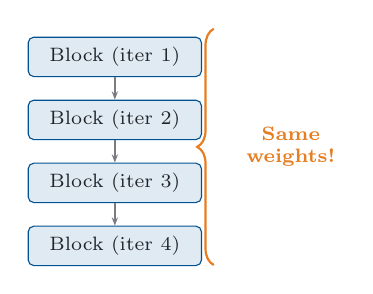
\begin{tikzpicture}[
        blk/.style={rectangle, draw=UnifiBlue, fill=UnifiBlue!12,
                    rounded corners=2pt, minimum width=2.2cm, minimum height=0.5cm,
                    font=\scriptsize, text=UnifiDark},
        arr/.style={-{Stealth[length=3pt]}, thick, UnifiDark!60}
      ]
        \node[blk] (b1) at (0,0)    {Block (iter 1)};
        \node[blk] (b2) at (0,-0.8) {Block (iter 2)};
        \node[blk] (b3) at (0,-1.6) {Block (iter 3)};
        \node[blk] (b4) at (0,-2.4) {Block (iter 4)};
        \draw[arr] (b1) -- (b2);
        \draw[arr] (b2) -- (b3);
        \draw[arr] (b3) -- (b4);
        % Shared weight indicator
        \draw[thick, AccentOrange, decorate, decoration={brace, amplitude=6pt, mirror}]
          (b1.north east) ++(0.15,0.1) -- ++(0,-3.0)
          node[midway, right=8pt, font=\scriptsize\bfseries, text=AccentOrange, align=center]{Same\\weights!};
      \end{tikzpicture}
      \end{center}

      \vspace{0.3em}
      \begin{table}
        \centering\scriptsize
        \begin{tabular}{lc}
          \toprule
          \textbf{Configuration} & \textbf{Parameters} \\
          \midrule
          Unshared ($T\!=\!4$ iters) & $\sim$8.67M \\
          \textbf{Shared ($T$ iterations)} & \textbf{$\sim$3.35M} \\
          \midrule
          Reduction & \alert{$\sim\!2.6\times$} \\
          \bottomrule
        \end{tabular}
      \end{table}
    \end{column}
  \end{columns}
\end{frame}

% ── Slide 9: Fourier Positional Encoding ─────────────────────────────────────
\begin{frame}[shrink=5]{Fourier Positional Encoding}
  \begin{columns}[T]
    \begin{column}{0.50\textwidth}
      \textbf{Why is it needed?}
      \begin{itemize}
        \item Attention is \textit{permutation-equivariant}
        \item Without PE the model has no notion of ``where'' data is
        \item Experimentally confirmed: \alert{61.34\% without PE} vs 72.02\% with PE
      \end{itemize}

      \vspace{0.5em}
      \textbf{Fourier PE} (per axis $x_d$, raw coord.\ concatenated):
      \[
      \gamma(x_d) = \bigl[\,x_d,\; \sin(f_k \pi x_d),\, \cos(f_k \pi x_d)\,\bigr]_{k=1}^{K}
      \]

      $K=64$ frequencies \textbf{linearly spaced} in $[1,\, \mu/2]$ ($\mu/2$ = Nyquist).
    \end{column}
    \begin{column}{0.46\textwidth}
      \textbf{Resulting dimensions:}

      \vspace{0.5em}
      \begin{table}
        \centering\small
        \begin{tabular}{lcc}
          \toprule
          \textbf{Modality} & \textbf{Pos. features} & \textbf{$C_{\text{tot}}$} \\
          \midrule
          Image (2D) & $3 + 2(2K{+}1)$ & $\mathbf{261}$ \\
          Points (3D) & $3 + 3(2K{+}1)$ & $\mathbf{390}$ \\
          Text (byte) & $128 + 64$ & $\mathbf{192}$ \\
          \bottomrule
        \end{tabular}
      \end{table}

      \vspace{0.5em}
      \begin{alertblock}{Critical Finding}
        Positional encoding is the \textbf{single most important} component: removing it costs \textbf{$-10.68$pp} ($72.02\% \to 61.34\%$).
      \end{alertblock}
    \end{column}
  \end{columns}
\end{frame}

% ── Slide 10: Perceiver IO Decoder ───────────────────────────────────────────
\begin{frame}[shrink=5]{Perceiver Forward Pass: Shape Checkpoints}
  \begin{columns}[T]
    \begin{column}{0.52\textwidth}
      \textbf{Data flow in the original Perceiver:}
      \begin{enumerate}
        \item Input is flattened and enriched:
        \[
          X=[\text{content}\,\|\,\gamma(\text{position})]\in\mathbb{R}^{M\times C_{\text{tot}}}
        \]
        \item Learned latent array:
        \[
          L_0\in\mathbb{R}^{N\times D},\qquad N\ll M
        \]
        \item Cross-attention reads input:
        \[
          Q=L W_Q,\quad K=XW_K,\quad V=XW_V
        \]
        \item Latent Transformer applies self-attention + FFN only on $N$ latents.
      \end{enumerate}
    \end{column}
    \begin{column}{0.44\textwidth}
      \textbf{ImageNet reference shapes:}
      \begin{table}
        \centering\scriptsize
        \begin{tabular}{lll}
          \toprule
          \textbf{Object} & \textbf{Shape} & \textbf{Meaning} \\
          \midrule
          $X$ & $50{,}176\times261$ & pixels + Fourier PE \\
          $L_0$ & $512\times1024$ & learned latents \\
          $Q$ & $512\times261$ & latent queries \\
          $K,V$ & $50{,}176\times261$ & input keys/values \\
          $A$ & $512\times50{,}176$ & attention map \\
          \bottomrule
        \end{tabular}
      \end{table}

      \vspace{0.4em}
      \begin{block}{Core idea}
        The input size $M$ affects only the cross-attention read; depth is spent in the compact latent space.
      \end{block}
    \end{column}
  \end{columns}
\end{frame}

% ── Slide 11: Output Query Design per Task ───────────────────────────────────
\begin{frame}[shrink=5]{Original Perceiver Output: Pooling Classifier}
  \begin{columns}[T]
    \begin{column}{0.49\textwidth}
      \textbf{Fixed-shape output head:}
      \[
        L_T=\mathrm{Encoder}(X,L_0)
      \]
      \[
        z=\frac{1}{N}\sum_{i=1}^{N}L_T[i]
      \]
      \[
        \mathrm{logits}=zW_{\mathrm{cls}}+b_{\mathrm{cls}}
      \]

      \vspace{0.4em}
      \begin{itemize}
        \item Mean pooling collapses all latents to one vector
        \item The classifier predicts one global label
        \item This is ideal for classification, not dense structured outputs
      \end{itemize}
    \end{column}
    \begin{column}{0.47\textwidth}
      \small
      \textbf{Where FFN and sharing fit:}
      \begin{itemize}
        \item Each latent block is pre-norm attention, residual, FFN, residual
        \item FFN adds non-linearity after attention mixing
        \item Weight sharing repeats the processor over iterations
      \end{itemize}

      \vspace{0.35em}
      \begin{alertblock}{Exam distinction}
        Perceiver IO replaces pooling with decoder cross-attention driven by output queries.
      \end{alertblock}
    \end{column}
  \end{columns}
\end{frame}

% ── Slide 12: Computational Complexity ───────────────────────────────────────
\begin{frame}{Computational Complexity Analysis}
  \begin{table}
    \centering\small
    \begin{tabular}{lccc}
      \toprule
      \textbf{Model} & \textbf{Self-Attn} & \textbf{Cross-Attn} & \textbf{Total} \\
      \midrule
      Standard Transformer & $\mathcal{O}(M^2 d)$ & --- & $\mathcal{O}(M^2 d \cdot L)$ \\
      \midrule
      Perceiver & $\mathcal{O}(N^2 d)$ & $\mathcal{O}(MNd)$ & $\mathcal{O}((MN + N^2 L)\,d)$ \\
      \bottomrule
    \end{tabular}
  \end{table}

  \vspace{0.5em}
  \begin{columns}[T]
    \begin{column}{0.48\textwidth}
      \textbf{Concrete example (CIFAR-10):}
      \begin{itemize}
        \item $M = 1024$ (pixels, $32{\times}32$), $N = 96$, $L = 4$
        \item Standard: $1024^2 = 1{,}048{,}576$
        \item Perceiver: $1024 \times 96 + 96^2 \times 4 = 135{,}168$
        \item \alert{$\sim\!7.8\times$ reduction}
      \end{itemize}
    \end{column}
    \begin{column}{0.48\textwidth}
      \textbf{Scaling advantage:}
      \begin{itemize}
        \item For images $224\!\times\!224$: $M\!=\!50k$
        \item Transformer: $2.5 \times 10^9$ ops
        \item Perceiver ($N\!=\!512$): $\sim\!26$M ops
        \item \alert{$\sim\!100\times$ reduction}
      \end{itemize}
    \end{column}
  \end{columns}
\end{frame}

% ── Slide 13: GELU & LAMB Optimizer ──────────────────────────────────────────
\begin{frame}[shrink=5]{GELU Activation \& LAMB Optimizer}
  \begin{columns}[T,onlytextwidth]
    \begin{column}{0.48\textwidth}
      \small
      \textbf{GELU (Gaussian Error Linear Unit):}
      \[
      \text{GELU}(x) = x \cdot \Phi(x) \approx x \cdot \sigma(1.702\,x)
      \]
      \vspace{-0.25em}
      \begin{itemize}
        \item Smooth activation used in Transformer architectures
        \item Allows small negative gradient flow
      \end{itemize}

      \vspace{0.2em}
      \textbf{LAMB (Layer-wise Adaptive Moments):}
      \vspace{-0.25em}
      \[
      r_t^{(l)} = \frac{\|w_t^{(l)}\|}{\|w_t^{(l)} + \eta\, \hat{u}_t^{(l)}\|}
      \]
      \vspace{-0.55em}
      {\footnotesize Per-layer trust ratio rescales updates and stabilizes large-batch training.}
    \end{column}
    \begin{column}{0.48\textwidth}
      \small
      \textbf{Why LAMB for Perceiver?}
      \begin{itemize}
        \item Cross-attention bottleneck creates high variance gradients
        \item Standard Adam can \alert{destabilize} with large batches
        \item LAMB safely scales batch sizes up to 1024
      \end{itemize}

      \vspace{0.25em}
      \begin{table}
        \centering\scriptsize
        \begin{tabular}{lcc}
          \toprule
          \textbf{Optimizer} & \textbf{Large Batches} & \textbf{Layer-wise LR} \\
          \midrule
          Adam & Diverges & Global \\
          \textbf{LAMB} & \textbf{Stable} & \textbf{Per-layer trust} \\
          \bottomrule
        \end{tabular}
      \end{table}
    \end{column}
  \end{columns}
\end{frame}

% ── Slide 14: Implementation ─────────────────────────────────────────────────
\begin{frame}[shrink=5]{Implementation}
  \vspace{0.15em}
  \begin{table}
    \centering\scriptsize
    \begin{tabular}{p{0.18\textwidth}p{0.36\textwidth}p{0.36\textwidth}}
      \toprule
      \textbf{Aspect} & \textbf{Paper implementation} & \textbf{Project code} \\
      \midrule
      Core model &
      Cross-attention into learned latents, latent self-attention, FFN, weight sharing &
      Same modules; weight sharing is exposed as an ablation switch \\
      \midrule
      Model scale &
      Large vision/language runs: up to $512{\times}1024$ latents and 201M-param IO &
      Smaller runs: CIFAR-10 $96{\times}384$, ModelNet40/text $128{\times}512$ \\
      \midrule
      Data setting &
      ImageNet, ModelNet40, large language pretraining corpora &
      CIFAR-10, ModelNet40, WikiText-103 byte-level MLM, GLUE fine-tuning \\
      \midrule
      Training budget &
      Distributed accelerators, batches up to 512--1024 &
      Single-GPU budget, batches 32--128, LAMB retained for stability \\
      \midrule
      Practical additions &
      Minimal regularization in the reference setup &
      Dropout, logging, attention-map extraction, and reproducible ablations \\
      \bottomrule
    \end{tabular}
  \end{table}

  \vspace{0.25em}
  {\small The implementation keeps the architectural mechanism intact; the main differences are scale, data budget and training resources.}
\end{frame}

% ══════════════════════════════════════════════════════════════════════════════
% SECTION 3: Experiments & Results (slides 15-28)
% ══════════════════════════════════════════════════════════════════════════════
\section{Perceiver Experiments \& Results}

% ── Slide 15: CIFAR-10 Setup ─────────────────────────────────────────────────
\begin{frame}[shrink=5]{CIFAR-10: Experimental Setup}
  \textbf{Goal:} validate the Perceiver on raw pixels without any CNN assumptions.

  \vspace{0.3em}
  \begin{columns}[T]
    \begin{column}{0.48\textwidth}
      \begin{table}
        \centering\small
        \begin{tabular}{ll}
          \toprule
          \textbf{Hyperparameter} & \textbf{Value} \\
          \midrule
          Latent dim ($N \times D$) & $96 \times 384$ \\
          Cross-attn stages & 4 \\
          Transformer blocks & 4 (shared) \\
          Attention heads & 3 \\
          Patch size & $2 \times 2$ \\
          Dropout & 0.2 \\
          \midrule
          Optimizer & LAMB \\
          Learning rate & 0.004 \\
          Batch size & 64 \\
          Epochs & 120 \\
          \midrule
          \textbf{Total parameters} & \textbf{$\sim$3.35M} \\
          \bottomrule
        \end{tabular}
      \end{table}
    \end{column}
    \begin{column}{0.48\textwidth}
      \textbf{Ablation study plan:}
      \begin{enumerate}
        \item Impact of positional encoding
        \item Weight sharing vs no sharing
        \item Robustness to pixel permutation
        \item Best classifier-head configuration
      \end{enumerate}

      \vspace{0.5em}
      \textbf{Data pipeline:}
      \begin{itemize}
        \item $32\!\times\!32$ RGB images, pixel-level input ($M\!=\!1024$)
        \item 2D Fourier positional encoding ($K\!=\!64$)
        \item Standard augmentation: horizontal flip, random crop
      \end{itemize}
    \end{column}
  \end{columns}
\end{frame}

% ── Slide 16: CIFAR-10 Ablation Results ──────────────────────────────────────
\begin{frame}[shrink=5]{CIFAR-10: Ablation Results}
  \begin{columns}[T]
    \begin{column}{0.50\textwidth}
      \begin{center}
      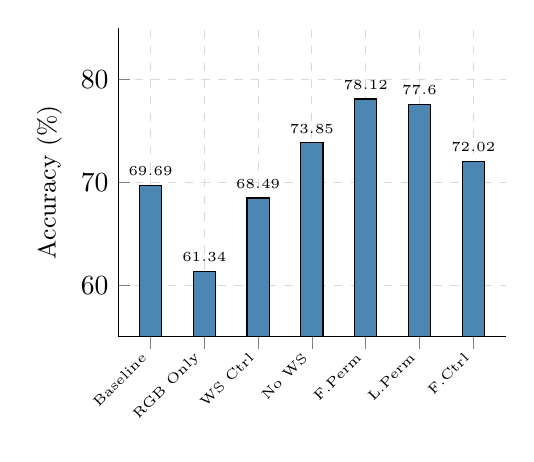
\begin{tikzpicture}
        \begin{axis}[
          ybar,
          width=6.5cm, height=5.5cm,
          bar width=8pt,
          ymin=55, ymax=85,
          ylabel={\small Accuracy (\%)},
          ylabel style={font=\small},
          symbolic x coords={Baseline,RGB Only,WS Ctrl,No WS,F.Perm,L.Perm,F.Ctrl},
          xtick=data,
          x tick label style={rotate=45, anchor=east, font=\tiny},
          nodes near coords,
          nodes near coords style={font=\tiny, above},
          every node near coord/.append style={rotate=0},
          enlarge x limits=0.1,
          grid=major,
          grid style={dashed, gray!30},
          axis lines*=left,
        ]
          \addplot[fill=UnifiBlue!70] coordinates {
            (Baseline, 69.69)
            (RGB Only, 61.34)
            (WS Ctrl, 68.49)
            (No WS, 73.85)
            (F.Perm, 78.12)
            (L.Perm, 77.60)
            (F.Ctrl, 72.02)
          };
        \end{axis}
      \end{tikzpicture}
      \end{center}
    \end{column}
    \begin{column}{0.46\textwidth}
      \begin{table}
        \centering\scriptsize
        \begin{tabular}{lc}
          \toprule
          \textbf{Experiment} & \textbf{Acc.} \\
          \midrule
          \textbf{Fourier Permuted} & \textbf{78.12\%} \\
          Learned PE Permuted & 77.60\% \\
          No Weight Sharing & 73.85\% \\
          Fourier Control & 72.02\% \\
          Baseline Fourier & 69.69\% \\
          WS Control & 68.49\% \\
          \textcolor{AccentRed}{\textbf{RGB Only (no PE)}} & \textcolor{AccentRed}{\textbf{61.34\%}} \\
          \bottomrule
        \end{tabular}
      \end{table}

      \vspace{0.3em}
      \textbf{Key observations:}
      \begin{itemize}
        \item PE is \alert{essential}: $-$10.68pp without it
        \item Permuted-pixel runs are \alert{best} (78.12\%), not worst
        \item Weight sharing: $-$5.36pp but $\sim$2.6$\times$ fewer params
      \end{itemize}
    \end{column}
  \end{columns}
\end{frame}

% ── Slide 17: PE Impact ──────────────────────────────────────────────────────
\begin{frame}[shrink=12]{CIFAR-10: Impact of Positional Encoding}
  \begin{columns}[T]
    \begin{column}{0.50\textwidth}
      \begin{center}
      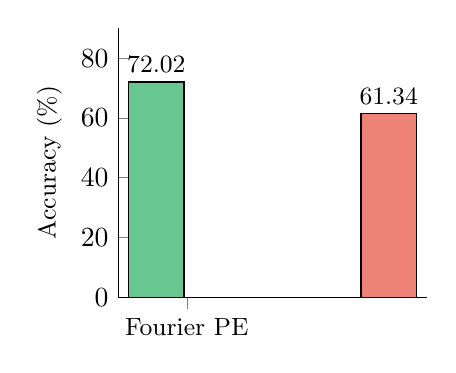
\begin{tikzpicture}
        \begin{axis}[
          ybar,
          width=5.5cm, height=5cm,
          bar width=20pt,
          ymin=0, ymax=90,
          ylabel={\small Accuracy (\%)},
          symbolic x coords={Fourier PE, No PE},
          xtick=data,
          x tick label style={font=\small},
          nodes near coords,
          nodes near coords style={font=\small\bfseries},
          enlarge x limits=0.4,
          axis lines*=left,
        ]
          \addplot[fill=AccentGreen!70] coordinates {(Fourier PE, 72.02)};
          \addplot[fill=AccentRed!70] coordinates {(No PE, 61.34)};
        \end{axis}
      \end{tikzpicture}
      \end{center}
    \end{column}
    \begin{column}{0.46\textwidth}
      \textbf{Why does this happen?}
      \begin{itemize}
        \item Attention is \textit{permutation-equivariant}
        \item Without PE the model cannot exploit spatial positions
        \item Color-only signal still classifies, but clearly weaker
      \end{itemize}

      \vspace{0.5em}
      \textbf{Quantitative impact:}
      \begin{itemize}
        \item With Fourier PE: \textbf{72.02\%}
        \item Without PE (RGB only): \textbf{61.34\%}
        \item Delta: \alert{$-$10.68 percentage points}
        \item Still well above chance (10\%), but markedly worse
      \end{itemize}

      \vspace{0.3em}
      This confirms the original paper's hypothesis that PE is the most critical component.
    \end{column}
  \end{columns}
\end{frame}

% ── Slide 18: Weight Sharing ─────────────────────────────────────────────────
\begin{frame}[shrink=5]{CIFAR-10: Weight Sharing Analysis}
  \begin{columns}[T]
    \begin{column}{0.48\textwidth}
      \textbf{Comparison:}
      \begin{table}
        \centering\small
        \begin{tabular}{lcc}
          \toprule
          \textbf{Config} & \textbf{Params} & \textbf{Acc.} \\
          \midrule
          Shared (baseline) & 3.35M & 69.69\% \\
          WS Control & 3.35M & 68.49\% \\
          \textbf{No Sharing} & \textbf{8.67M} & \textbf{73.85\%} \\
          \bottomrule
        \end{tabular}
      \end{table}

      \vspace{0.5em}
      \textbf{Trade-off:}
      \begin{itemize}
        \item No sharing: $+$5.36pp accuracy
        \item But $\sim$2.6$\times$ more parameters
        \item Efficiency ratio: $\sim$1.0pp per 1M extra params
      \end{itemize}
    \end{column}
    \begin{column}{0.48\textwidth}
      \textbf{Why weight sharing works:}
      \begin{itemize}
        \item Acts like a \textit{recurrent} processor in latent space
        \item Iterative refinement of representations
        \item Implicit regularization effect
        \item Critical for deployment on limited hardware
      \end{itemize}

      \vspace{0.5em}
      \begin{block}{Practical Implication}
        Weight sharing reaches \textbf{92.7\%} of the no-sharing accuracy with only \textbf{39\%} of the parameters --- a strong efficiency trade-off for resource-constrained scenarios.
      \end{block}
    \end{column}
  \end{columns}
\end{frame}

% ── Slide 19: Permutation Robustness ─────────────────────────────────────────
\begin{frame}[shrink=5]{CIFAR-10: Permutation Robustness}
  \begin{columns}[T]
    \begin{column}{0.48\textwidth}
      \textbf{Experiment:} train \emph{and} evaluate on pixels shuffled by a single fixed permutation $\sigma$ (same $\sigma$ throughout).

      \vspace{0.5em}
      \begin{table}
        \centering\small
        \begin{tabular}{lc}
          \toprule
          \textbf{Configuration} & \textbf{Acc.} \\
          \midrule
          Fourier PE (natural order) & 69.69\% \\
          \textbf{Fourier PE (permuted)} & \textbf{78.12\%} \\
          Learned PE (permuted) & 77.60\% \\
          \bottomrule
        \end{tabular}
      \end{table}

      \vspace{0.3em}
      \textbf{Counterintuitive result:}
      \begin{itemize}
        \item Permuting pixels \alert{raises} accuracy: $+$8.43pp
        \item Fourier vs learned (permuted): $+$0.52pp
      \end{itemize}
    \end{column}
    \begin{column}{0.48\textwidth}
      \textbf{Analysis:}
      \begin{itemize}
        \item The Perceiver has \textbf{no built-in 2D bias}: position is read only from the PE
        \item With a fixed $\sigma$ in train \emph{and} test, it learns the layout from the Fourier features alone
        \item \textbf{Fourier PE} (deterministic) slightly beats learned PE and generalizes better
      \end{itemize}

      \vspace{0.5em}
      \begin{alertblock}{Insight}
        Permutation invariance is a \textbf{feature}, not a weakness: the model assumes nothing about input ordering, exactly as the paper argues (Jaegle et al., 2021, Tab.~2).
      \end{alertblock}
    \end{column}
  \end{columns}
\end{frame}

% ── Slide 20: Perceiver vs Perceiver IO ──────────────────────────────────────
\begin{frame}{CIFAR-10: Best Perceiver Configuration}
  \begin{columns}[T]
    \begin{column}{0.48\textwidth}
      \begin{center}
      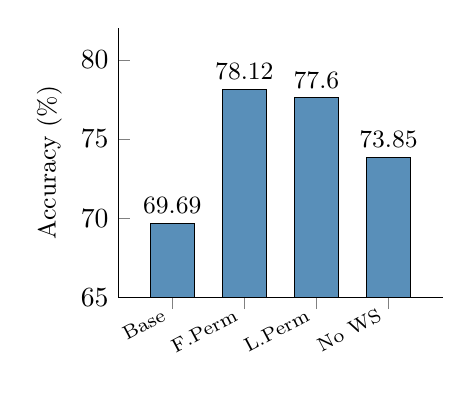
\begin{tikzpicture}
        \begin{axis}[
          ybar,
          width=5.7cm, height=5cm,
          bar width=16pt,
          ymin=65, ymax=82,
          ylabel={\small Accuracy (\%)},
          symbolic x coords={Base,F.Perm,L.Perm,No WS},
          xtick=data,
          x tick label style={rotate=28, anchor=east, font=\scriptsize},
          nodes near coords,
          nodes near coords style={font=\small\bfseries},
          enlarge x limits=0.25,
          axis lines*=left,
        ]
          \addplot[fill=UnifiBlue!65] coordinates {
            (Base,69.69)
            (F.Perm,78.12)
            (L.Perm,77.60)
            (No WS,73.85)
          };
        \end{axis}
      \end{tikzpicture}
      \end{center}
    \end{column}
    \begin{column}{0.48\textwidth}
      \textbf{Best Perceiver result:}
      \begin{table}
        \centering\small
        \begin{tabular}{lc}
          \toprule
          \textbf{Configuration} & \textbf{Acc.} \\
          \midrule
          \textbf{Fourier PE, permuted} & \textbf{78.12\%} \\
          Learned PE, permuted & 77.60\% \\
          No weight sharing & 73.85\% \\
          Baseline Fourier & 69.69\% \\
          \bottomrule
        \end{tabular}
      \end{table}

      \vspace{0.35em}
      {\small
      \textbf{Takeaway:}
      \begin{itemize}
        \item Fourier PE carries the spatial signal explicitly.
        \item Weight sharing is an efficiency--accuracy trade-off.
      \end{itemize}
      }
    \end{column}
  \end{columns}
\end{frame}

% ── Slide 21: ModelNet40 Setup & Results ─────────────────────────────────────
\begin{frame}[shrink=5]{ModelNet40: Setup \& Results}
  \begin{columns}[T]
    \begin{column}{0.48\textwidth}
      \textbf{Configuration:}
      \begin{table}
        \centering\small
        \begin{tabular}{ll}
          \toprule
          \textbf{Hyperparameter} & \textbf{Value} \\
          \midrule
          Latent dim ($N \times D$) & $128 \times 512$ \\
          Cross-attn stages & 2 \\
          Transformer blocks & 6 (shared) \\
          Points per object & 2048 \\
          Optimizer & LAMB \\
          Epochs & 200 \\
          Batch size & 128 \\
          \bottomrule
        \end{tabular}
      \end{table}
    \end{column}
    \begin{column}{0.48\textwidth}
      \textbf{Results:}
      \begin{table}
        \centering\small
        \begin{tabular}{lc}
          \toprule
          \textbf{Configuration} & \textbf{Acc.} \\
          \midrule
          \textbf{Baseline (scale)} & \textbf{84.24\%} \\
          + Translation & 83.67\% \\
          + Rotation & 83.14\% \\
          \midrule
          \textit{Original Paper} & \textit{85.7\%} \\
          \bottomrule
        \end{tabular}
      \end{table}

      \vspace{0.3em}
      \begin{exampleblock}{Excellent Reproduction}
        Gap of only \textbf{1.46pp} vs the original paper, despite using batch size 128 vs 512 (GPU constraints).
      \end{exampleblock}
    \end{column}
  \end{columns}
\end{frame}

% ── Slide 22: ModelNet40 Augmentation ─────────────────────────────────────────
\begin{frame}[shrink=15]{ModelNet40: Augmentation Effects}
  \begin{columns}[T]
    \begin{column}{0.50\textwidth}
      \begin{center}
      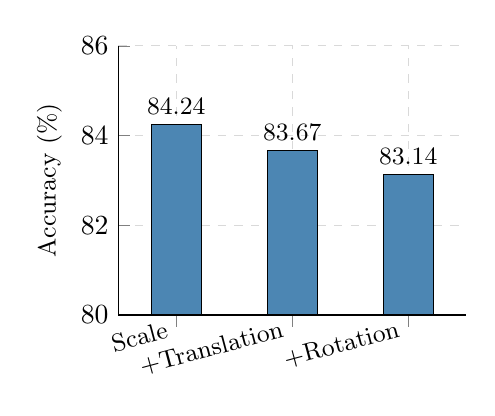
\begin{tikzpicture}
        \begin{axis}[
          ybar,
          width=6cm, height=5cm,
          bar width=18pt,
          ymin=80, ymax=86,
          ylabel={\small Accuracy (\%)},
          symbolic x coords={Scale, +Translation, +Rotation},
          xtick=data,
          x tick label style={rotate=15, anchor=east, font=\small},
          nodes near coords,
          nodes near coords style={font=\small\bfseries},
          enlarge x limits=0.25,
          axis lines*=left,
          grid=major,
          grid style={dashed, gray!30},
        ]
          \addplot[fill=UnifiBlue!70] coordinates {
            (Scale, 84.24)
            (+Translation, 83.67)
            (+Rotation, 83.14)
          };
        \end{axis}
      \end{tikzpicture}
      \end{center}
    \end{column}
    \begin{column}{0.46\textwidth}
      \textbf{Analysis:}
      \begin{itemize}
        \item \textbf{Scale only} (baseline): best result at 84.24\%
        \item Adding translation: $-$0.57pp
        \item Adding rotation: $-$1.10pp
      \end{itemize}

      \vspace{0.5em}
      \textbf{Why augmentation doesn't help:}
      \begin{itemize}
        \item With 3D Fourier PE the Perceiver already handles rotations natively
        \item So rotation augmentation is \emph{redundant} --- adds noise, not signal
        \item ModelNet40 objects are already centred, limiting translation's effect
      \end{itemize}

      \vspace{0.3em}
      \textbf{Comparison with paper (85.7\%):}\\
      Gap due to batch size (128 vs 512) and fewer training resources.
    \end{column}
  \end{columns}
\end{frame}

% ── Slide 23: WikiText-103 MLM Pre-training ──────────────────────────────────
\section{Perceiver IO}

% -- Perceiver IO: Structured Outputs ------------------------------------------------
\begin{frame}[shrink=5]{Perceiver IO: Structured Outputs}
  \begin{center}
    
\includegraphics[width=0.70\textwidth,height=0.30\textheight,keepaspectratio]{perceiver_io_architecture.png}
  \end{center}

  \vspace{0.15em}
  \begin{columns}[T,onlytextwidth]
    \begin{column}{0.48\textwidth}
      \small
      \textbf{Extension over Perceiver} (Jaegle et al., ICLR 2022):
      \begin{itemize}
        \item \textbf{Encode}: input $\rightarrow$ latent (same cross-attn encoder)
        \item \textbf{Process}: latent self-attention ($\times L$)
        \item \textbf{Decode}: \alert{output queries} read latents
      \end{itemize}
    \end{column}
    \begin{column}{0.48\textwidth}
      \small
      \textbf{Why it matters:}
      \begin{itemize}
        \item Original Perceiver: one pooled global output
        \item IO: task-specific output shape
        \item Same latent bottleneck, more general decoder
      \end{itemize}
    \end{column}
  \end{columns}
\end{frame}

% -- Perceiver IO Decoder ------------------------------------------------------------
\begin{frame}[shrink=12]{Perceiver IO Decoder with Output Queries}
  \begin{center}
    
\includegraphics[width=0.86\textwidth,height=0.31\textheight,keepaspectratio]{perceiver_io_decoder.png}
  \end{center}

  \vspace{0.25em}
  \textbf{Decoder cross-attention (single layer):}
  \[
  Q_{\text{dec}} = \text{OutputQuery}\,W_Q, \quad
  K_{\text{dec}} = \text{Latent}\,W_K, \quad
  V_{\text{dec}} = \text{Latent}\,W_V
  \]
  \[
  \text{Output} = \text{softmax}\!\left(\frac{Q_{\text{dec}} K_{\text{dec}}^\top}{\sqrt{d_k}}\right) V_{\text{dec}} \in \mathbb{R}^{O \times E}
  \]

  \vspace{0.3em}
  \begin{itemize}
    \item The number of output queries $O$ is \textbf{task-dependent} and independent of $N$ and $M$
    \item A single decoder cross-attention layer suffices (no self-attention among outputs)
  \end{itemize}
\end{frame}

% -- Output Query Design -------------------------------------------------------------
\begin{frame}[shrink=5]{Output Query Design per Task}
  \begin{center}
    
\includegraphics[width=0.95\textwidth,height=0.42\textheight,keepaspectratio,trim=150 365 150 90,clip]{output_queries.png}
  \end{center}

  \vspace{-0.15em}
  \begin{columns}[T,onlytextwidth]
    \begin{column}{0.31\textwidth}
      \begin{block}{Classification}
        \scriptsize One learned query; decoder projection produces class logits.
      \end{block}
    \end{column}
    \begin{column}{0.31\textwidth}
      \begin{block}{Dense outputs}
        \scriptsize One query per target position, e.g. pixels or voxels.
      \end{block}
    \end{column}
    \begin{column}{0.31\textwidth}
      \begin{block}{Masked LM}
        \scriptsize Masked byte positions query logits over the 256-byte vocabulary.
      \end{block}
    \end{column}
  \end{columns}

  \vspace{-0.1em}
  \begin{center}
    \scriptsize Output queries define what the decoder reads from the latent array.
  \end{center}
\end{frame}

% -- CIFAR comparison after IO explanation ------------------------------------------
\begin{frame}[shrink=5]{CIFAR-10: Perceiver vs Perceiver IO}
  \begin{columns}[T]
    \begin{column}{0.48\textwidth}
      \begin{center}
      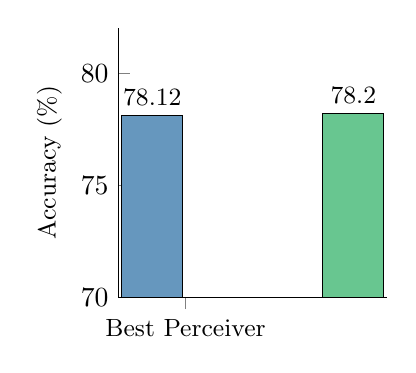
\begin{tikzpicture}
        \begin{axis}[
          ybar,
          width=5cm, height=5cm,
          bar width=22pt,
          ymin=70, ymax=82,
          ylabel={\small Accuracy (\%)},
          symbolic x coords={Best Perceiver,Perceiver IO},
          xtick=data,
          x tick label style={font=\small},
          nodes near coords,
          nodes near coords style={font=\small\bfseries},
          enlarge x limits=0.5,
          axis lines*=left,
        ]
          \addplot[fill=UnifiBlue!60] coordinates {(Best Perceiver,78.12)};
          \addplot[fill=AccentGreen!70] coordinates {(Perceiver IO,78.20)};
        \end{axis}
      \end{tikzpicture}
      \end{center}
    \end{column}
    \begin{column}{0.48\textwidth}
      \textbf{Why the decoder helps:}
      \begin{itemize}
        \item Output query is a learned aggregation instead of fixed mean pooling
        \item Decoder cross-attention attends selectively to relevant latents
        \item Small gain on CIFAR-10, but same mechanism enables MLM and dense outputs
        \item Cost: $\sim$3$\times$ parameters (9.5M vs 3.35M)
      \end{itemize}

      \vspace{0.4em}
      \begin{table}
        \centering\small
        \begin{tabular}{lcc}
          \toprule
          \textbf{Model} & \textbf{Acc.} & \textbf{$\Delta$} \\
          \midrule
          Best Perceiver & 78.12\% & --- \\
          \textbf{Perceiver IO} & \textbf{78.20\%} & \textcolor{AccentGreen}{\textbf{+0.08pp}} \\
          \bottomrule
        \end{tabular}
      \end{table}
    \end{column}
  \end{columns}
\end{frame}

\begin{frame}[shrink=5]{WikiText-103: Masked Language Model Pre-training}
  \textbf{Goal:} pre-train a general language encoder without specialized tokenizers.

  \vspace{0.3em}
  \begin{columns}[T]
    \begin{column}{0.48\textwidth}
      \begin{table}
        \centering\small
        \begin{tabular}{ll}
          \toprule
          \textbf{Component} & \textbf{Detail} \\
          \midrule
          Tokenization & Byte-level (UTF-8) \\
          Vocabulary size & 256 \\
          Sequence length & 1024 \\
          Mask probability & 15\% \\
          Model & Perceiver IO ($\sim$10M) \\
          Epochs / batch & 50 / 32 \\
          \midrule
          \textbf{Masked byte acc.} & \textbf{82.20\%} \\
          \bottomrule
        \end{tabular}
      \end{table}
    \end{column}
    \begin{column}{0.48\textwidth}
      \textbf{Why byte-level?}
      \begin{itemize}
        \item No BPE/WordPiece tokenizer needed
        \item Truly language-agnostic input
        \item Fixed vocabulary of size 256
        \item Trade-off: longer sequences for same text
      \end{itemize}

      \vspace{0.5em}
      \textbf{MLM task:}
      \begin{itemize}
        \item 15\% of byte positions masked
        \item Output queries = masked positions
        \item Decoder predicts original byte values
        \item Cross-entropy loss over 256 classes
      \end{itemize}
    \end{column}
  \end{columns}
\end{frame}

% ── Slide 24: GLUE Fine-tuning ───────────────────────────────────────────────
\begin{frame}[shrink=5]{GLUE: Fine-tuning on 8 Tasks}
  \begin{columns}[T,onlytextwidth]
    \begin{column}{0.34\textwidth}
      \textbf{Transfer pipeline:}

      \vspace{0.4em}
      \begin{center}
        
\includegraphics[width=\textwidth,height=0.46\textheight,keepaspectratio]{byte_latent_arrays.png}
      \end{center}
    \end{column}
    \begin{column}{0.62\textwidth}
      \textbf{Fine-tuning setup:}
      \begin{itemize}
        \item Transfer pre-trained MLM encoder
        \item Replace output queries with classification query
        \item 30 epochs, LR = $5 \times 10^{-4}$
        \item Byte-level input (same as pre-training)
      \end{itemize}

      \vspace{0.2em}
      \textbf{8 GLUE benchmark tasks:}
      \begin{itemize}
        \item \textbf{Single sentence:} CoLA, SST-2
        \item \textbf{Similarity:} MRPC, STS-B, QQP
        \item \textbf{Inference:} MNLI, QNLI, RTE
      \end{itemize}

      \vspace{0.15em}
      Each task tests a different NLU capability with the same architecture.
    \end{column}
  \end{columns}
\end{frame}

% ── Slide 25: GLUE Per-Task Analysis ─────────────────────────────────────────
\begin{frame}[shrink=8]{GLUE: Per-Task Analysis}
  \begin{columns}[T]
    \begin{column}{0.55\textwidth}
      \begin{center}
        
\includegraphics[width=\textwidth,height=0.55\textheight,keepaspectratio]{glue_chart.png}
      \end{center}
    \end{column}
    \begin{column}{0.42\textwidth}
      \textbf{Key observations:}
      \begin{itemize}
        \item \textbf{QQP} (paraphrase): best task at 75.65\%
        \item \textbf{CoLA} 69.13\%, \textbf{MRPC} 68.38\% follow
        \item \textbf{MNLI} (46.47\%) \& \textbf{RTE} (52.71\%): hardest --- need deep NLI reasoning
        \item Mean $\sim$63\% vs paper $\sim$81\%
      \end{itemize}

      \vspace{0.3em}
      \textbf{Limitations:}
      \begin{itemize}
        \item Byte-level tokenization produces long sequences
        \item Smaller model ($\sim$10M) vs paper's IO (201M)
        \item No subword semantics available
      \end{itemize}
    \end{column}
  \end{columns}
\end{frame}

% ── Slide 26: Convergence ────────────────────────────────────────────────────
\begin{frame}[shrink=5]{Convergence: All Experiments}
  \begin{columns}[T]
    \begin{column}{0.55\textwidth}
      \begin{center}
        
\includegraphics[width=\textwidth,height=0.55\textheight,keepaspectratio]{convergence_chart.png}
      \end{center}
    \end{column}
    \begin{column}{0.42\textwidth}
      \textbf{Convergence speed by modality:}

      \vspace{0.3em}
      \begin{table}
        \centering\small
        \begin{tabular}{lc}
          \toprule
          \textbf{Modality} & \textbf{Epochs} \\
          \midrule
          Point Clouds & $\sim$50 (fast) \\
          Text (GLUE FT) & $\sim$15--30 \\
          Images (CIFAR-10) & $\sim$120 (slow) \\
          \bottomrule
        \end{tabular}
      \end{table}

      \vspace{0.3em}
      \textbf{Observations:}
      \begin{itemize}
        \item Point clouds: low-dimensional input, fast convergence
        \item GLUE: transfer learning accelerates training
        \item CIFAR-10: pixel-level input requires many iterations for spatial learning
      \end{itemize}
    \end{column}
  \end{columns}
\end{frame}

% ── Slide 27: Attention Maps ─────────────────────────────────────────────────
\begin{frame}[shrink=25]{Attention Maps Analysis}
  \begin{columns}[T]
    \begin{column}{0.48\textwidth}
      \begin{center}
        \textbf{Fourier PE (Epoch 81)}\\[2pt]
        
\includegraphics[width=0.9\textwidth,height=0.45\textheight,keepaspectratio]{exp1_baseline_fourier_evolution.png}
      \end{center}

      \vspace{0.2em}
      {\small Structured, spatially selective patterns (entropy $\sim$6.4). Latents specialize in different image regions.}
    \end{column}
    \begin{column}{0.48\textwidth}
      \begin{center}
        \textbf{RGB Only --- no PE (Epoch 81)}\\[2pt]
        
\includegraphics[width=0.9\textwidth,height=0.45\textheight,keepaspectratio]{exp3B_rgb_only_evolution.png}
      \end{center}

      \vspace{0.2em}
      {\small Diffuse, near-uniform patterns (entropy $\sim$9.1). No spatial selectivity --- the model cannot localize information.}
    \end{column}
  \end{columns}

  \vspace{0.3em}
  \begin{block}{Interpretation}
    With Fourier PE, cross-attention learns spatially coherent patterns across training.
    Without PE, attention entropy remains high and patterns lack structure.
  \end{block}
\end{frame}

% ── Slide 28: Comprehensive Results Summary ──────────────────────────────────
\begin{frame}[shrink=5]{Comprehensive Results Summary}
  \begin{table}
    \centering\small
    \begin{tabular}{llccl}
      \toprule
      \textbf{Modality} & \textbf{Model} & \textbf{Best Acc.} & \textbf{Paper} & \textbf{Experiments} \\
      \midrule
      Images (CIFAR-10) & Perceiver & 78.12\% & $>$90\% & 7 ablations \\
      Images (CIFAR-10) & Perceiver IO & \textbf{78.20\%} & --- & 1 \\
      Point Clouds (ModelNet40) & Perceiver & 84.24\% & 85.7\% & 3 augmentations \\
      Text (WikiText-103) & Perceiver IO & 82.20\% MLM & --- & 1 \\
      NLU (GLUE, 8 tasks) & Perceiver IO & $\sim$63\% avg & --- & 8 fine-tuning \\
      \bottomrule
    \end{tabular}
  \end{table}

  \vspace{0.5em}
  \begin{columns}[T]
    \begin{column}{0.48\textwidth}
      \textbf{Highlights:}
      \begin{itemize}
        \item ModelNet40: only 1.46pp gap from paper
        \item Perceiver IO slightly edges the best Perceiver
        \item Successful transfer MLM $\rightarrow$ GLUE
      \end{itemize}
    \end{column}
    \begin{column}{0.48\textwidth}
      \textbf{Overall numbers:}
      \begin{itemize}
        \item $\sim$2500 lines of PyTorch code
        \item 20+ distinct training runs
        \item 3 modalities: 2D images, 3D points, text
        \item 100\% reproducible via \texttt{reproduce.py}
      \end{itemize}
    \end{column}
  \end{columns}
\end{frame}

% ══════════════════════════════════════════════════════════════════════════════
% SECTION 4: Criticalities & Discussion (slides 29-33)
% ══════════════════════════════════════════════════════════════════════════════
\section{Criticalities \& Discussion}

% ── Slide 29: Gap vs Original Paper ──────────────────────────────────────────
\begin{frame}[shrink=10]{Gap vs Original Paper}
  \begin{columns}[T]
    \begin{column}{0.48\textwidth}
      \textbf{ModelNet40 (Point Clouds):}
      \begin{table}
        \centering\small
        \begin{tabular}{lc}
          \toprule
          \textbf{Source} & \textbf{Acc.} \\
          \midrule
          Original Paper & 85.7\% \\
          Our Implementation & 84.24\% \\
          \midrule
          \textbf{Gap} & \textcolor{AccentGreen}{\textbf{1.46pp}} \\
          \bottomrule
        \end{tabular}
      \end{table}

      \vspace{0.3em}
      \textcolor{AccentGreen}{\textbf{Excellent reproduction.}}\\
      Small gap attributable to reduced batch size (128 vs 512).
    \end{column}
    \begin{column}{0.48\textwidth}
      \textbf{CIFAR-10 (Images):}
      \begin{table}
        \centering\small
        \begin{tabular}{lc}
          \toprule
          \textbf{Source} & \textbf{Acc.} \\
          \midrule
          Original Paper & $>$90\% \\
          Our Perceiver IO & 78.20\% \\
          \midrule
          \textbf{Gap} & \textcolor{AccentRed}{\textbf{$\sim$12pp}} \\
          \bottomrule
        \end{tabular}
      \end{table}

      \vspace{0.3em}
      \textcolor{AccentRed}{\textbf{Significant gap.}}\\
      Caused by hardware constraints: 512 TPU cores vs single consumer GPU.
    \end{column}
  \end{columns}

  \vspace{0.5em}
  \begin{block}{Root Cause Analysis}
    The CIFAR-10 gap is primarily due to \textbf{batch size} (64 vs 1024), \textbf{latent count} (96 vs 256), and \textbf{compute time} limitations. The Perceiver architecture is particularly sensitive to these scaling factors on image data.
  \end{block}
\end{frame}

% ── Slide 30: Hardware Limitations ───────────────────────────────────────────
\begin{frame}[shrink=8]{Hardware Limitations \& Design Choices}
  \begin{table}
    \centering\small
    \begin{tabular}{lcc}
      \toprule
      \textbf{Parameter} & \textbf{Original Paper (Google)} & \textbf{Our Setup} \\
      \midrule
      Hardware & 512 TPU v3 cores & 1 NVIDIA consumer GPU \\
      Batch size & up to 1024 & max 64--128 \\
      Latents ($N$) & 256--512 & 96--128 \\
      Model size & 30--100M+ params & 3.35--10M params \\
      Training time & days (distributed) & hours--days (single GPU) \\
      \bottomrule
    \end{tabular}
  \end{table}

  \vspace{0.5em}
  \begin{columns}[T]
    \begin{column}{0.48\textwidth}
      \textbf{Consequences:}
      \begin{itemize}
        \item LAMB optimizer less effective with small batches
        \item Fewer latents limit representational capacity
        \item Reduced augmentation due to time constraints
        \item Fewer hyperparameter search iterations
      \end{itemize}
    \end{column}
    \begin{column}{0.48\textwidth}
      \textbf{Mitigation strategies:}
      \begin{itemize}
        \item Weight sharing to reduce memory
        \item Gradient accumulation where possible
        \item Careful cosine annealing schedule
        \item Focus experiments on most informative ablations
      \end{itemize}
    \end{column}
  \end{columns}
\end{frame}

% ── Slide 31: Possible Improvements ──────────────────────────────────────────
\begin{frame}[shrink=9]{Possible Improvements}
  \begin{columns}[T]
    \begin{column}{0.48\textwidth}
      \textbf{Architecture:}
      \begin{itemize}
        \item Increase latent count ($N = 256$+) with gradient checkpointing
        \item Add multi-scale cross-attention (coarse $\rightarrow$ fine)
        \item Explore relative positional encodings (RoPE, ALiBi)
        \item Deeper decoder for structured outputs
      \end{itemize}

      \vspace{0.5em}
      \textbf{Training:}
      \begin{itemize}
        \item Larger batch sizes with gradient accumulation
        \item Mixed precision (FP16/BF16) training
        \item Longer training schedules
        \item Advanced augmentation (CutMix, MixUp)
      \end{itemize}
    \end{column}
    \begin{column}{0.48\textwidth}
      \textbf{Data \& Tasks:}
      \begin{itemize}
        \item ImageNet pre-training for vision
        \item Subword tokenization for NLP
        \item Multi-modal joint training
        \item Audio modality experiments
      \end{itemize}

      \vspace{0.5em}
      \textbf{Analysis:}
      \begin{itemize}
        \item Layer-wise attention probing
        \item Latent space clustering visualization
        \item Systematic hyperparameter search
        \item Comparison with efficient Transformers (Linformer, Performer)
      \end{itemize}
    \end{column}
  \end{columns}
\end{frame}

% ── Slide 32: Lessons Learned ────────────────────────────────────────────────
\begin{frame}[shrink=5]{Lessons Learned}
  \begin{columns}[T]
    \begin{column}{0.48\textwidth}
      \textbf{What works well:}
      \begin{itemize}
        \item Genuinely \alert{modality-agnostic} architecture
        \item Weight sharing: $\sim$2.6$\times$ fewer parameters, modest accuracy cost
        \item Perceiver IO slightly edges base Perceiver on CIFAR-10
        \item Transfer learning MLM $\rightarrow$ GLUE is effective
        \item Fourier PE is robust and general-purpose
      \end{itemize}
    \end{column}
    \begin{column}{0.48\textwidth}
      \textbf{Observed limitations:}
      \begin{itemize}
        \item Performance gap vs paper on images ($\sim$12pp)
        \item LAMB optimizer sensitive to batch size
        \item Byte-level tokenization produces very long sequences for text
        \item Augmentation can hurt with limited training
        \item Hyperparameter tuning is time-consuming
      \end{itemize}
    \end{column}
  \end{columns}

  \vspace{0.5em}
  \begin{block}{Main Takeaway}
    \textbf{Positional encoding} is the single most critical component of the architecture: without it, accuracy drops from 72\% to 61\% on CIFAR-10, confirming the paper's core hypothesis.
  \end{block}
\end{frame}

% ── Slide 33: Conclusions ────────────────────────────────────────────────────
\begin{frame}[shrink=15]{Conclusions}
  \begin{columns}[T]
    \begin{column}{0.48\textwidth}
      \textbf{Strengths of the Perceiver:}
      \begin{itemize}
        \item Single architecture for images, point clouds, and text
        \item Linear complexity in input size
        \item Strong memory efficiency via weight sharing ($\sim$61\%)
        \item Zero CNN/RNN domain-specific assumptions
        \item Output queries enable flexible structured decoding
      \end{itemize}
    \end{column}
    \begin{column}{0.48\textwidth}
      \textbf{Weaknesses:}
      \begin{itemize}
        \item Requires large compute to match specialized models
        \item Heavily depends on positional encoding
        \item Outperformed by efficient CNNs on standard vision benchmarks
        \item LAMB optimizer introduces training instability at small scale
        \item Latent bottleneck limits fine-grained spatial reasoning
      \end{itemize}
    \end{column}
  \end{columns}

  \vspace{0.5em}
  \begin{exampleblock}{Final Assessment}
    The Perceiver demonstrates that a \textbf{single general-purpose architecture} can handle diverse modalities. While it does not yet match domain-specific models at limited scale, the paradigm is a compelling step toward truly modality-agnostic perception.
  \end{exampleblock}
\end{frame}

% ══════════════════════════════════════════════════════════════════════════════
% SECTION 5: Closing (slides 34-36)
% ══════════════════════════════════════════════════════════════════════════════
\section{Closing}

% ── Slide 34: References ─────────────────────────────────────────────────────
\begin{frame}{References}
  \small
  \begin{thebibliography}{9}
    \bibitem{perceiver} A.~Jaegle et al.,
    \textit{Perceiver: General Perception with Iterative Attention},
    ICML 2021.

    \bibitem{perceiverio} A.~Jaegle et al.,
    \textit{Perceiver IO: A General Architecture for Structured Inputs \& Outputs},
    ICLR 2022.

    \bibitem{attention} A.~Vaswani et al.,
    \textit{Attention Is All You Need},
    NeurIPS 2017.

    \bibitem{lamb} Y.~You et al.,
    \textit{Large Batch Optimization for Deep Learning: Training BERT in 76 Minutes},
    ICLR 2020.

    \bibitem{fourierfeatures} M.~Tancik et al.,
    \textit{Fourier Features Let Networks Learn High Frequency Functions in Low Dimensional Domains},
    NeurIPS 2020.

    \bibitem{geglu} N.~Shazeer,
    \textit{GLU Variants Improve Transformer},
    arXiv 2020.
  \end{thebibliography}
\end{frame}

% ── Slide 35: Appendix – Expected Questions ──────────────────────────────────
\begin{frame}{Appendix: Expected Questions}
  \begin{columns}[T]
    \begin{column}{0.48\textwidth}
      \textbf{Architecture:}
      \begin{enumerate}
        \item Why cross-attention instead of full self-attention?\\
          {\scriptsize $\rightarrow$ Reduces $\mathcal{O}(M^2)$ to $\mathcal{O}(NM)$}
        \item How does weight sharing affect performance?\\
          {\scriptsize $\rightarrow$ $-$5.36pp for $\sim$2.6$\times$ fewer params}
        \item Why Fourier PE over learned PE?\\
          {\scriptsize $\rightarrow$ More robust to permutation, generalizes better}
        \item What is the role of GEGLU?\\
          {\scriptsize $\rightarrow$ Higher non-linear capacity, stable gradients}
      \end{enumerate}
    \end{column}
    \begin{column}{0.48\textwidth}
      \textbf{Experiments:}
      \begin{enumerate}\setcounter{enumi}{4}
        \item Why is the CIFAR-10 gap so large?\\
          {\scriptsize $\rightarrow$ Hardware limits: batch 64 vs 1024, 96 vs 256 latents}
        \item Why byte-level tokenization for NLP?\\
          {\scriptsize $\rightarrow$ Truly modality-agnostic, no external tokenizer}
        \item How does Perceiver IO improve on Perceiver?\\
          {\scriptsize $\rightarrow$ Learned output queries vs mean pooling}
        \item Could this replace ViT/BERT?\\
          {\scriptsize $\rightarrow$ Not yet at limited scale; promising at Google scale}
      \end{enumerate}
    \end{column}
  \end{columns}
\end{frame}

% ── Slide 36: Thank You ──────────────────────────────────────────────────────
\begin{frame}
  \begin{center}
    {\Huge\color{UnifiBlue}\textbf{Thank you!}}\\[1.5em]
    {\Large\color{UnifiDark} Questions?}\\[2.5em]
    {\color{UnifiDark}Francesco Gigli e Corso Vignoli}\\[0.3em]
    {\small\color{UnifiDark} Code and models available upon request}\\[1.5em]
    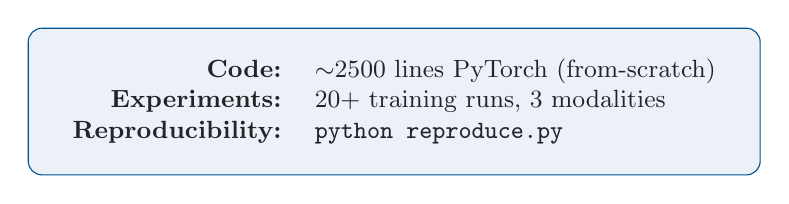
\begin{tikzpicture}
      \node[rectangle, draw=UnifiBlue, fill=UnifiBlue!8, rounded corners=5pt,
            inner sep=10pt, font=\small, text=UnifiDark] {
        \begin{tabular}{rl}
          \textbf{Code:} & $\sim$2500 lines PyTorch (from-scratch) \\
          \textbf{Experiments:} & 20+ training runs, 3 modalities \\
          \textbf{Reproducibility:} & \texttt{python reproduce.py} \\
        \end{tabular}
      };
    \end{tikzpicture}
  \end{center}
\end{frame}

\end{document}
